\begin{figure}[H]
    \centering
    \begin{subfigure}{0.5\textwidth}
        \centering
        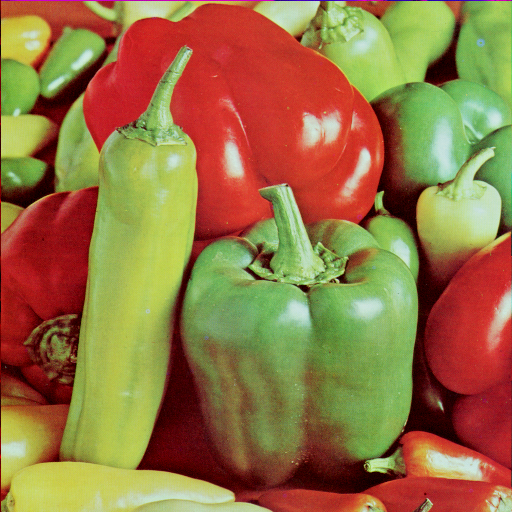
\includegraphics[width=0.85\textwidth]{mona_assin/imagem.png}
        \caption{Imagem com mensagem oculta.}
        \label{fig:assinatura:imagem}
    \end{subfigure}%
    \begin{subfigure}{0.5\textwidth}
        \centering
        \includegraphics[width=0.85\textwidth]{mona_assin/plano0.png}
        \caption{Plano 0.}
        \label{fig:assinatura:plano}
    \end{subfigure}\\[8pt]
    \begin{subfigure}{0.33\textwidth}
        \centering
        \includegraphics[width=0.85\textwidth]{mona_assin/pl0chb.png}
        \caption{Plano 0, canal azul.}
        \label{fig:assinatura:blue}
    \end{subfigure}%
    \begin{subfigure}{0.33\textwidth}
        \centering
        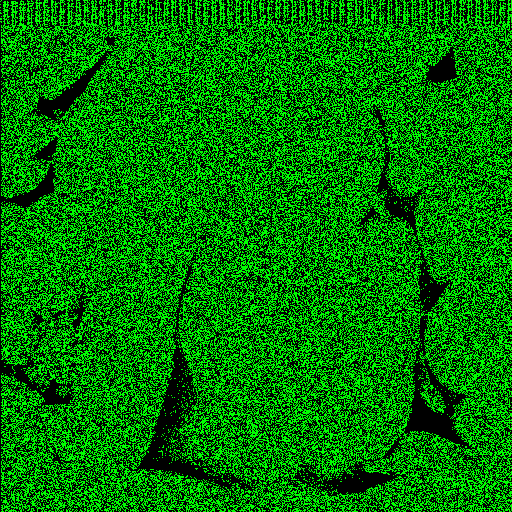
\includegraphics[width=0.85\textwidth]{mona_assin/pl0chg.png}
        \caption{Plano 0, canal verde.}
        \label{fig:assinatura:green}
    \end{subfigure}%
    \begin{subfigure}{0.33\textwidth}
        \centering
        \includegraphics[width=0.85\textwidth]{mona_assin/pl0chr.png}
        \caption{Plano 0, canal vermelho.}
        \label{fig:assinatura:red}
    \end{subfigure}%

    \caption{\texttt{monalisa.png} com uma assinatura de 35 bytes.}
    \label{fig:assinatura}
\end{figure}